\subsection{Team meetings and events}
\subsubsection{16.11.2015}
\begin{itemize}
\item Today it was assembled wheel base of the robot. The chain wasn't connected.
\begin{figure}[H]
	\begin{minipage}[h]{1\linewidth}
		\center{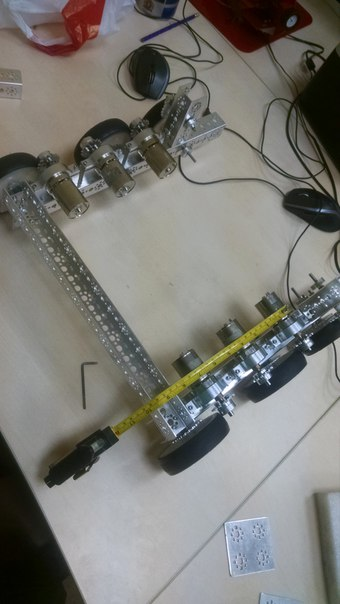
\includegraphics[scale=0.5]{days_L/Meetings/images/01}}
		\caption{Wheel base without chain}
	\end{minipage}
\end{figure} 
\item Also it was made the gripper with plastic bottle.
\begin{figure}[H]
	\begin{minipage}[h]{1\linewidth}
		\center{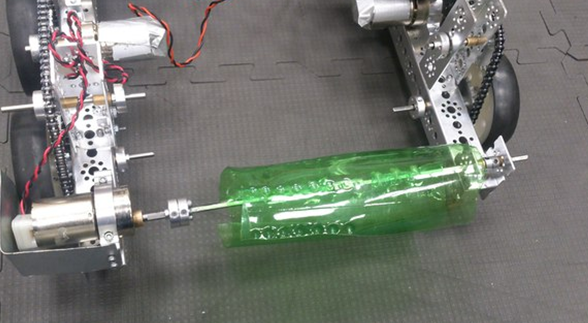
\includegraphics[scale=0.5]{days_L/Gripper/images/05}}
		\caption{Gripper with bottle}
	\end{minipage}
\end{figure}
\end{itemize}
\subsubsection{19.11.2015}
\begin{itemize}
\item Today the chains were connected to gears on the wheel base. It was wrote the programme for tele op and wheel base was tested on the field. Robot can move and turn fast and accurate
\begin{figure}[H]
	\begin{minipage}[h]{1\linewidth}
		\center{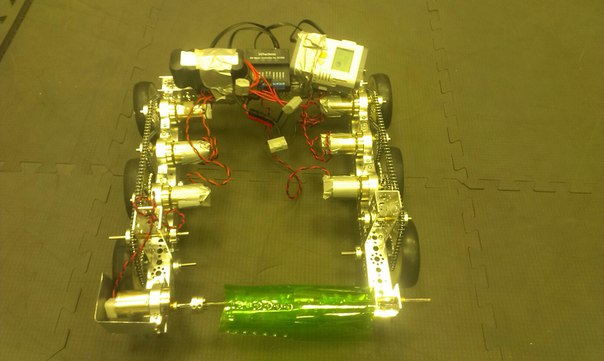
\includegraphics[scale=0.5]{days_L/Meetings/images/02}}
		\caption{Wheel base with chain}
	\end{minipage}
\end{figure} 
\item Also it was assembled the lift. But it wasn't installed on the robot.
\end{itemize}
\subsubsection{21.11.2015}
\begin{itemize}
\item The trainings with wheel base were continued. Also the mount for bucket was installed on the lift.
\end{itemize}
\subsubsection{23.11.2015}
\begin{itemize}
\item It was made and fixed on the lift bucket for debris. In addition the lift was installed to wheel base. 
\begin{figure}[H]
	\begin{minipage}[h]{1\linewidth}
		\center{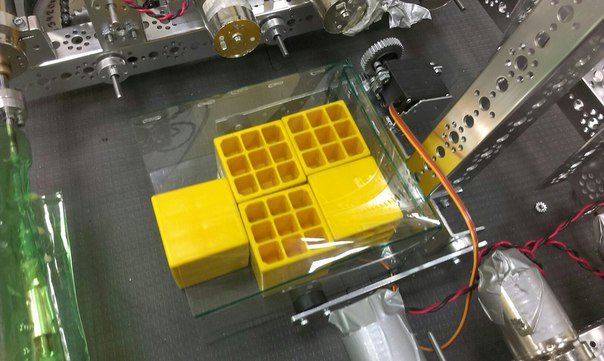
\includegraphics[scale=0.5]{days_L/Meetings/images/03}}
		\caption{The bucket for debris}
	\end{minipage}
\end{figure} 
\begin{figure}[H]
	\begin{minipage}[h]{1\linewidth}
		\center{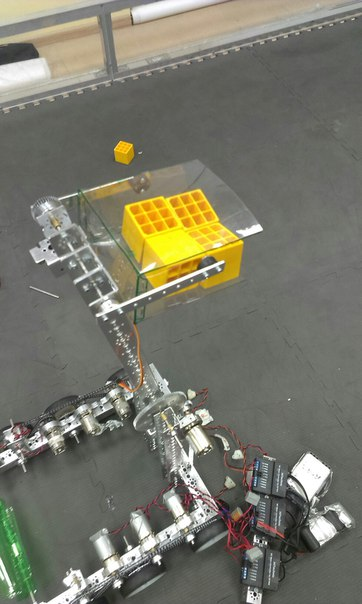
\includegraphics[scale=0.5]{days_L/Meetings/images/04}}
		\caption{The bucket on the rised position}
	\end{minipage}
\end{figure} 
\end{itemize}
\subsubsection{24.11.2015}
\begin{itemize}
\item It was found that gears on servo that turn bucket slip under the loads. So it was made the plate that doesn't allow to gears go away from each other. 
\item It was installed the cover for bucket.
\begin{figure}[H]
	\begin{minipage}[h]{1\linewidth}
		\center{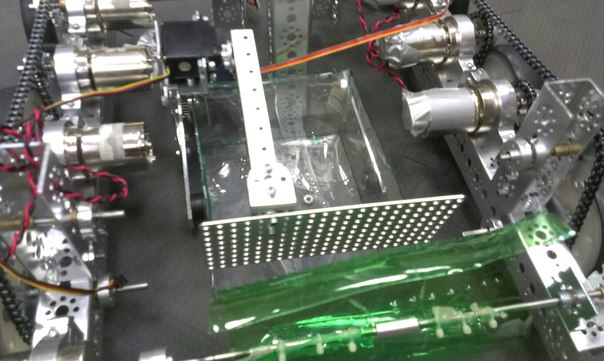
\includegraphics[scale=0.5]{days_L/Meetings/images/05}}
		\caption{Cover closed}
	\end{minipage}
\end{figure} 
\begin{figure}[H]
	\begin{minipage}[h]{1\linewidth}
		\center{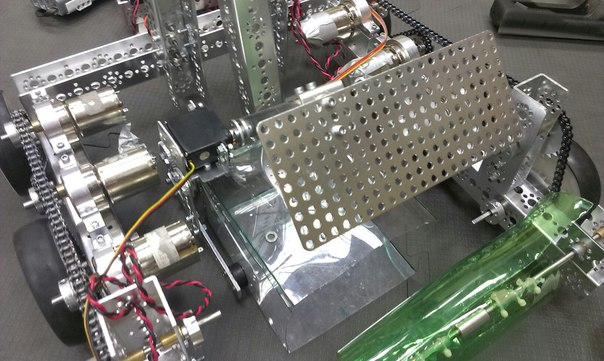
\includegraphics[scale=0.5]{days_L/Meetings/images/06}}
		\caption{Cover opened}
	\end{minipage}
\end{figure} 
\item Also they were cut the slopes for gripper.
\end{itemize}
\subsubsection{25.11.2015}
\begin{itemize}
\item The slopes were installed on the robot.
'\item Also today we bought the hose for gripper. 
\item Motor and servo controllers and NXT brick were installed on the robot.
\end{itemize}
\begin{figure}[H]
	\begin{minipage}[h]{1\linewidth}
		\center{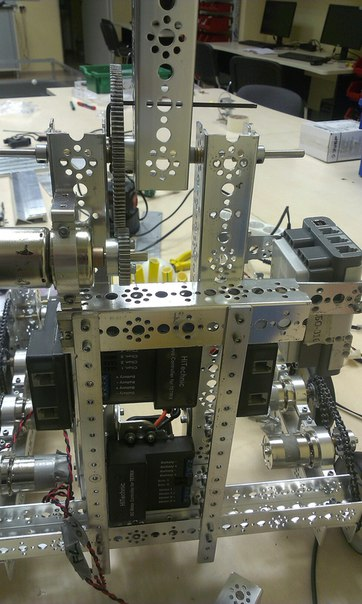
\includegraphics[scale=0.5]{days_L/Meetings/images/07}}
		\caption{Controllers}
	\end{minipage}
\end{figure} 
\subsubsection{26.11.2015}
\begin{itemize}
\item Today were hold wires of power for controllers.
\end{itemize}
\subsubsection{27.11.2015}
\begin{itemize}
\item The wiring of motors was hold.
\end{itemize}
\subsubsection{28.11.2015}
\begin{itemize}
\item It was found that the chain slip on back motors. So they were mounted so that chains touch larger sector of the gears that rotate by this motors.
\end{itemize}
\subsubsection{30.11.2015}
\begin{itemize}
\item The wires for servo were hold. Servos were set up. The programme for tele op was finished.
\item They were connected encoder of the motor that turn lift and encoder of the right side of wheel base. The left encoder of the wheel base wasn't connected because we had not enough wires for encoder. But if we need move on straight line or turn by both wheels pairs one encoder is enough.
\item The brush of gripper was remade.
\item Also we tested climbing to the ramp. It was found that robot can't do it because the front wheel is too long from edge of robot. So it was decided to score only to low box on the closest competition (5 - 6 of December). That is because we haven't enough time to remake something so it is better to train score to low box and write good autonomous period (score climbers and push button). In addition we tested how robot can score to middle box if it climb to low zone. It was found that it is very hard if we turn by the robot. So we need mechanism that turn bucket to the side. It was decided to make it after the competition. In addition it was found that it is difficult to ride to middle zone. So we need make mechanism that extend moving beam so that it can reach high box from low zone. But it was decided make it after competition too.
\item It was found that we can score bottom zip line climber if we push it by the bucket for debris. 
\end{itemize}
\subsubsection{01.12.2015}
\begin{itemize}
\item Today operators trained on the robot control. In this process it was found that screws that fix gears on motors get out. So they were fixed with help of sealant. 
\item During trainings we reached the next result: full low box in 2 minutes.
\end{itemize}
\subsubsection{02.12.2015}
\begin{itemize}
\item Today we were writing programme for autonomous period. It was wrote riding to the button and framework for pushing button. Now robot navigates by encoders. Also it was installed F-shaped beam.
\begin{figure}[H]
	\begin{minipage}[h]{1\linewidth}
		\center{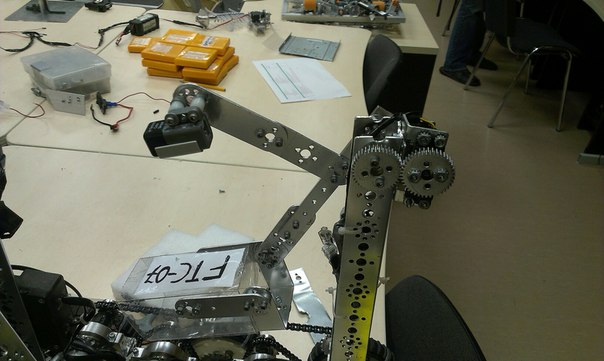
\includegraphics[scale=0.5]{days_L/Meetings/images/08}}
		\caption{F-shaped beam}
	\end{minipage}
\end{figure} 
\end{itemize}
\fillpage